\documentclass[11pt]{article} % use larger type; default would be 10pt

\usepackage{graphicx} % support the \includegraphics command and options

\title{Homogenization Notes}
\author{Giffin, B.}

\begin{document}
\maketitle

\section{Approach}

The goal of our approach is to model the propagation of crack networks caused by hydraluic fracturing using a homogenized representation of the physical reality. Rather than modeling individual geometric cracks within the rock, the presence and effects of cracks are approximated by a poroelastic solid medium permeated by a compressible fluid phase. For simplicity, only one fluid phase would be considered and surface tension forces would be neglected, but the medium itself would not necessarily be fully saturated. A representative volume element (RVE) with associated porosity and saturation would be utilized to develop a micromechanical model for use at the macroscopic level. The resulting problem would consist of two coupled problems: the deformation of the poroelastic medium, and the flow of the  incompressible, not fully saturated, single fluid phase through the porus medium. Governing equations for each of these phenomena are presented in section 3. In addition, the boundary conditions for each problem (on the solid, and on the fluid) would be independent of one another.

\subsection{Considerations}

\begin{itemize}
	\item[-] Representative volume element used to establish a continuum material
	\item[-] Single fluid phase
	\begin{itemize}
		\item[-] Not fully saturated (void space not occupied by fluid is assumed to have zero pressure; vaccum)
		\item[-] Compressible
	\end{itemize}
	\item[-] Poroelastic medium
	\begin{itemize}
		\item[-] Elastostatic equilibrium
		\item[-] Stress and strain averaged values over the solid ``skeleton'' in RVE
	\end{itemize}	
	\item[-] Evolve the porosity and hydraulic conductivity (anisotropically) to simulate facture propagation
	\item[-] Hydraulic conductivity increased in the plane defined by a `crack'' normal vector
	\item[-] Coupled solution of equations for deformation of solid and flow of fluid
\end{itemize}

\subsection{Advantages}

\begin{itemize}
	\item[-] Implementation would be relatively simple
	\item[-] Approach would work well given the scale of the problems being considered (large elements compared to size of cracks)
	\item[-] Could be easily adapted for any number of element types
	\item[-] Reduced preference for direction of crack propagation
	\item[-] No requirement for modeling physical crack geometry (eliminates the need for remeshing)
\end{itemize}

\section{List of Variables}

\subsection{General}

\begin{itemize}
	\item[$x$] Global position in cartesian coordinates (vector)
	\item[$t$] Time (scalar)
	\item[$g$] Gravitational body force (vector)
	\item[$\mathcal{V}$] RVE (spatial region occupied by a single exterior envelope)
\end{itemize}

\subsection{Poroelastic Solid}

\begin{itemize}
	\item[$\rho^s$] Solid phase density (scalar)
	\item[$\phi$] Porosity (scalar)
	\item[$K^w$] Bulk modulus of solid phase (scalar)
	\item[$C$] Macroscopic stiffness of solid (rank 4 tensor)
	\item[$E$] Microscopic stiffness of solid (rank 4 tensor)
	\item[$\bar{\mathcal{V}}$] Solid phase within RVE
	\item[$u$] Displacement (vector)
	\item[$T$] Macroscopic stress in solid (rank 2 tensor)
	\item[$e$] Macroscopic strain in solid (rank 2 tensor)
	\item[$\sigma$] Microscopic ``skelton'' stress in solid (rank 2 tensor)
	\item[$\epsilon$] Microscopic ``skelton'' strain in solid (rank 2 tensor)
\end{itemize}

\subsection{Compressible Fluid}

\begin{itemize}
	\item[$\mu$] Fluid viscosity (scalar)
	\item[$K^w$] Fluid bulk modulus (scalar)
	\item[$\rho^w$] Fluid density (scalar)
	\item[$v^w$] Fluid specific volume (scalar)
	\item[$S$] Fluid saturation (scalar)
	\item[$\kappa$] Hydraulic Conductivity/Permeability (rank 2 tensor)
	\item[$P$] Fluid pressure (scalar)
	\item[$m$] Fluid mass per unit volume in RVE (scalar)
	\item[$q$] Volume flux relative to solid (vector)
	\item[$Q$] Mass flux per unit volume in RVE, relative to solid (vector)
\end{itemize}

\section{Governing Equations}

\subsection{Equilibrium of Poroelastic Solid}

\begin{equation}
	\frac{\partial T_{ij}}{\partial x_j} - \rho^s \left( 1 - \phi \right) g = 0(??)
\end{equation}

\begin{equation}
	-\frac{T_{kk}}{3} =  K^s \left( \frac{1}{\rho^s} - \frac{1}{\rho^s_0} \right)
\end{equation}

\begin{equation}
	\phi = \frac{|\mathcal{V}| -  |\bar{\mathcal{V}}|}{|\mathcal{V}|} \in \left[ 0, 1 \right)
\end{equation}

\begin{equation}
	T_{ij} = \frac{1}{|\bar{\mathcal{V}}|} \int_{\bar{\mathcal{V}}} \sigma_{ij} dv
\end{equation}

\begin{equation}
	e_{ij} = \frac{1}{|\bar{\mathcal{V}}|} \int_{\bar{\mathcal{V}}} \epsilon_{ij} dv
\end{equation}

Displacement B.C.s: $u_i = \bar{u_i}$ on $\Gamma_u$

Traction B.C.s: $T_{ij} n_j = \bar{t_i}$ on $\Gamma_t$

\subsection{Compressible Fluid Flow in Porous Medium}

\begin{equation}
	q_i = \frac{\kappa_{ij}}{\mu}\left(-\frac{\partial P}{\partial x_j}+\rho^w g_j\right)
\end{equation}

\begin{equation}
	Q_i = \rho^w q_i
\end{equation}

\begin{equation}
	m = \rho^w \phi S
\end{equation}

\begin{equation}
	\frac{\partial m}{\partial t} = - \frac{\partial Q_i}{\partial x_i}
\end{equation}

\begin{equation}
	S \in \left[ 0, 1 \right]
\end{equation}

\begin{equation}
	f(S) \in \left[ 0, 1 \right]
\end{equation}

\begin{figure}
	\centering
	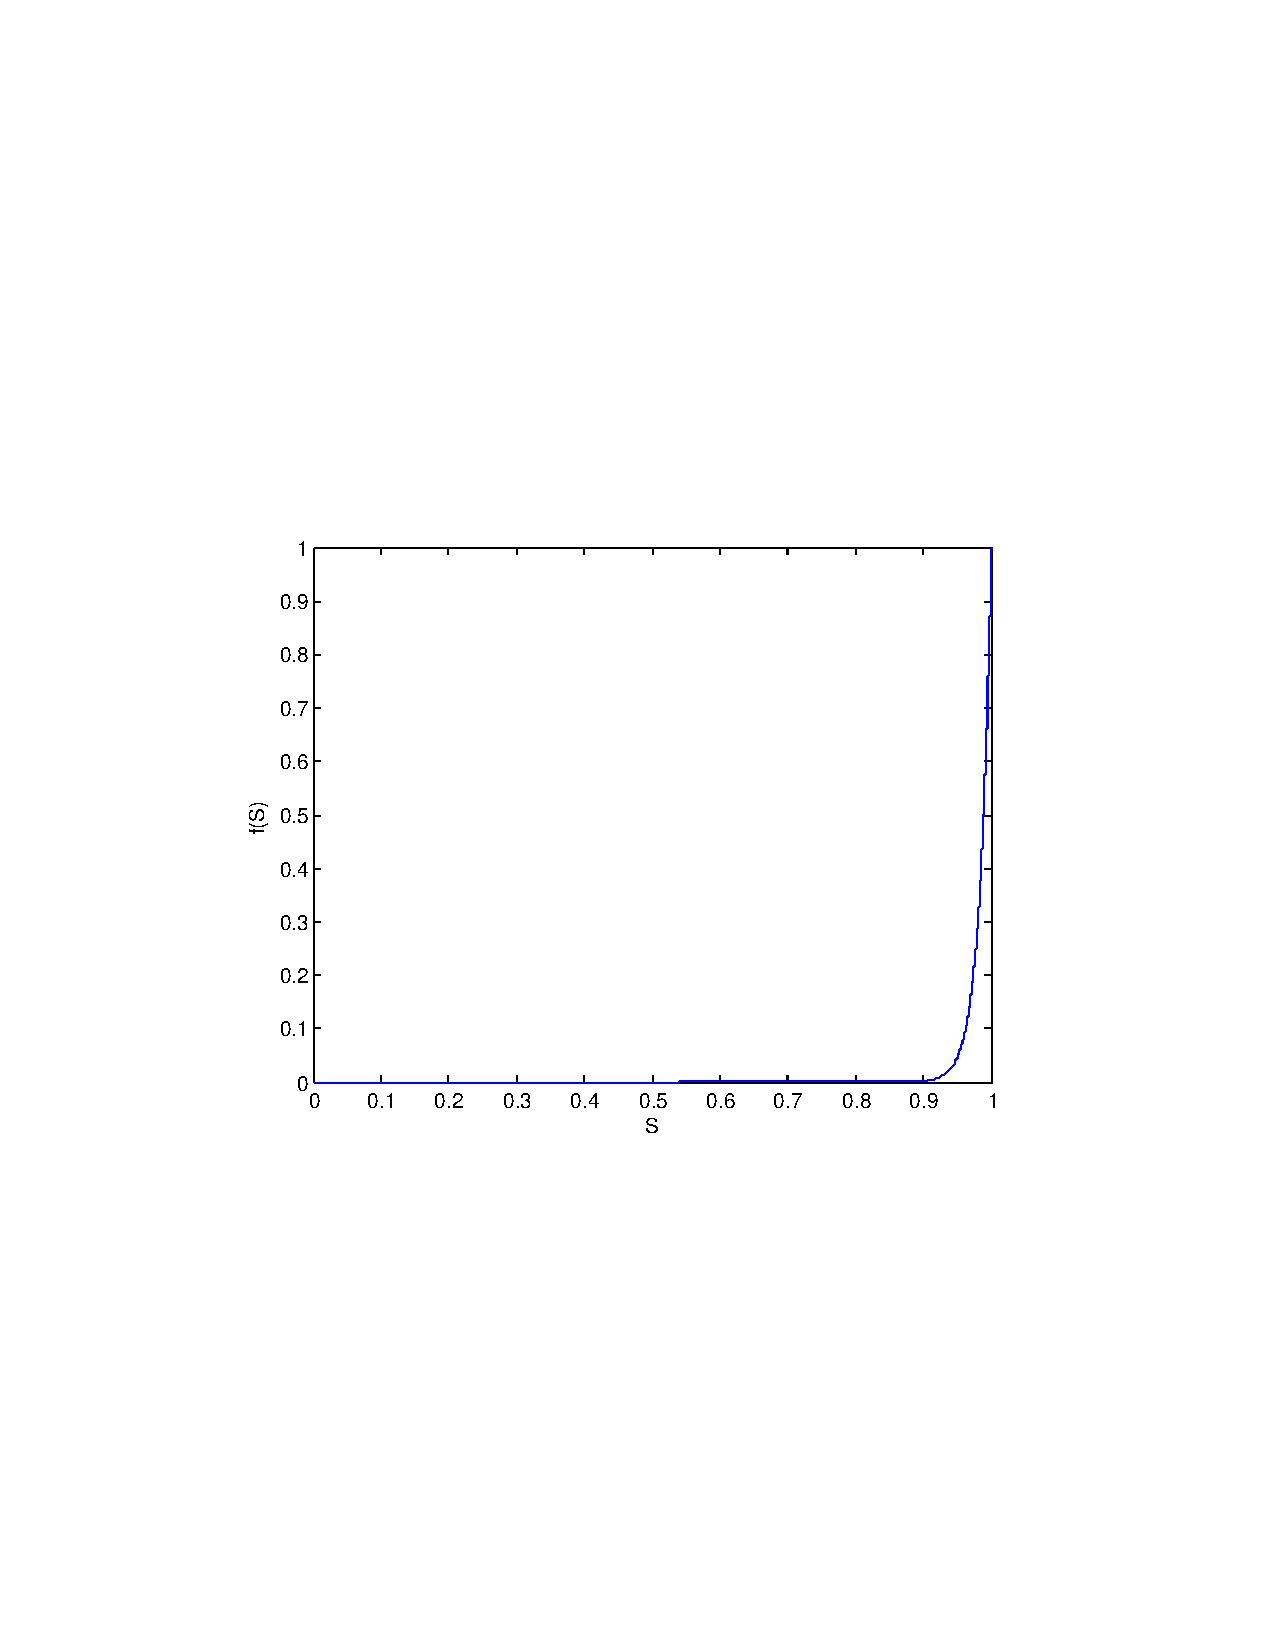
\includegraphics[width =4in,trim=110 240 130 240,clip=true]{fofs.pdf}
	\caption{$f(S)$ vs $S$ (Example: $f(S) = S^n$, for $n$ a natural number)}
\end{figure}

\begin{equation}
	P = K^w \left( v - v_0 \right) f(S) =  K^w \left( \frac{1}{\rho^w} - \frac{1}{\rho^w_0} \right) f(S)
\end{equation}

\begin{equation}
	e_{ij} = \frac{1}{|\bar{\mathcal{V}}|} \int_{\bar{\mathcal{V}}} \epsilon_{ij} dv
\end{equation}

Pressure B.C.s: $P = \bar{P}$ on $\Gamma_P$

Mass Flux B.C.s: $Q_i n_i = -\bar{\mathcal{Q}}$ on $\Gamma_\mathcal{Q}$

\newpage

\section{Questions Regarding Implementation}

\begin{itemize}
	\item[-] Is there a need to account for other fluid phases, in particular oil or gas?
	\item[-] What type of flow (saturated? number of fluid phases? compressible?) is considered for the current implementation?
	\item[-] How is this flow implemented in the code? Flow solvers? Coupled solution with equilibrium? Could these solvers be adapted for implementation into our homogenized approach?
	\item[-] Would our approach work best as a modification of an existing element type? Or solely as a change in the constitutive behavior of elements?
	\item[-] To what degree is paralleization of interest or concern?
	\item[-] Does GEOS use any external libraries? If so, to what degree must we be familiar with these libraries?
	\item[-] How often is GEOS updated? How would we go about obtaining a VotD? Would we need to?
	\item[-] How would we be able to share changes to the code without making serious (or potentially crippling) alterations to the GEOS repository?
	\item[-] How does one execute a GEOS problem from start to finish?
	\begin{itemize}
		\item[-] Mesh creation
		\item[-] Input deck format
		\item[-] Running on LC machines
		\item[-] Visualizing/interpreting results
		\item[-] Example problems?
	\end{itemize}
	\item[-] Are there any LC help resources specific to GEOS?
	\item[-] Other, more general, LC resources available to us?
	\item[-] Please describe the architecture of the code with respect to:
	\begin{itemize}
		\item[-] Linear algebra and tensor operations
		\item[-] Constitutive laws: material deformation and permeability?
		\item[-] Element types
		\item[-] Quadrature rules
		\item[-] Data structures
	\end{itemize}
	\item[-] Is there a preferred approach for making additions/alterations to the existing code? How have other adaptations/implementations been made?
\end{itemize}

\section{Additional Notes}

\end{document}